\documentclass[12pt]{article}
\usepackage[utf8]{inputenc}
\usepackage{geometry, amsmath, amsthm, latexsym, amssymb, graphicx, bm, pgfplots, float}
\usepackage{tikz}
\geometry{margin=1in, headsep=0.25in}

\parindent 0in
\parskip 12pt
\pgfplotsset{compat=1.17}

\begin{document}
\title{Exercício EAD0671}

%\thispagestyle{empty}

\begin{center}
    {\LARGE \bf Exercício 10} \\
    
    {\large Douglas Cardoso - 11766990}\\
EAD0671
\end{center}

\textbf{Ex. 10}\\
No Exemplo 9.1, calculamos ganhos e perdas decorrentes do controle de preços exercido sobre o gás natural e descobrimos a existência de um peso morto de US\$ 5,68 bilhões. Esse cálculo baseou-se em um preço de US\$ 50 por barril de petróleo.

(a) Se o preço do petróleo fosse de US\$ 70 por barril, qual seria o preço do gás natural no mercado livre? Qual seria o valor do peso morto resultante caso o preço máximo permitido para o gás natural fosse de US\$ 3 por mil pés cúbicos?

\begin{align*}
Oferta: Q^S = 15,90 + 0,72P_G + 0,05P_P \\
Demanda: Q^D = 0,02 - 1,8P_G + 0,69P_P
\end{align*}

Ao preço de \$70 por barril, o preço do gás natural no mercado livre é dado pelo seguinte cálculo:

\begin{gather*}
      Q^S = Q^D \\
    15,90 + 0,72P_G + 0,05 \times 70 = 0,02 - 1,8P_G + 0,69 \times 70 \\
    19,4 + 0,72P_G = 48,32 - 1,8P_G \\
    \bm{P_G = 11,4762}
\end{gather*}
 
A quantidade de equilíbrio a esse preço é de $\bm{27,66}$ - o cálculo foi feito substituindo o preço de equilíbrio na equação da oferta, e para validação, na equação da demanda.

Para a segunda questão, referente ao cálculo do peso morto quando fixa um preço para o gás natural de US\$ 3 mil por pés cúbicos, a nova quantidade de equilíbrio é de $\bm{21,56}$ para a oferta e $\bm{42,96}$ para a demanda - o preço que corta a curva de demanda com essa nova quantidade ofertada é de $\bm{14,86}$. Tendo esses números, a \textit{perda líquida excedente total} é dada por

\begin{gather*}
    B = (\frac{1}{2}) \times (27,6 - 21,56) \times (14,86 - 11,47) \\
    \bm{B = 10,2378} \\
    C = (\frac{1}{2}) \times (27,6 - 21,56) \times (11,47 - 3) \\
    C = \bm{25,5794} \\
    Peso\ morto = B + C \\
    \bm{Peso\ morto = 35,8172}
\end{gather*}

\begin{figure}[H]
    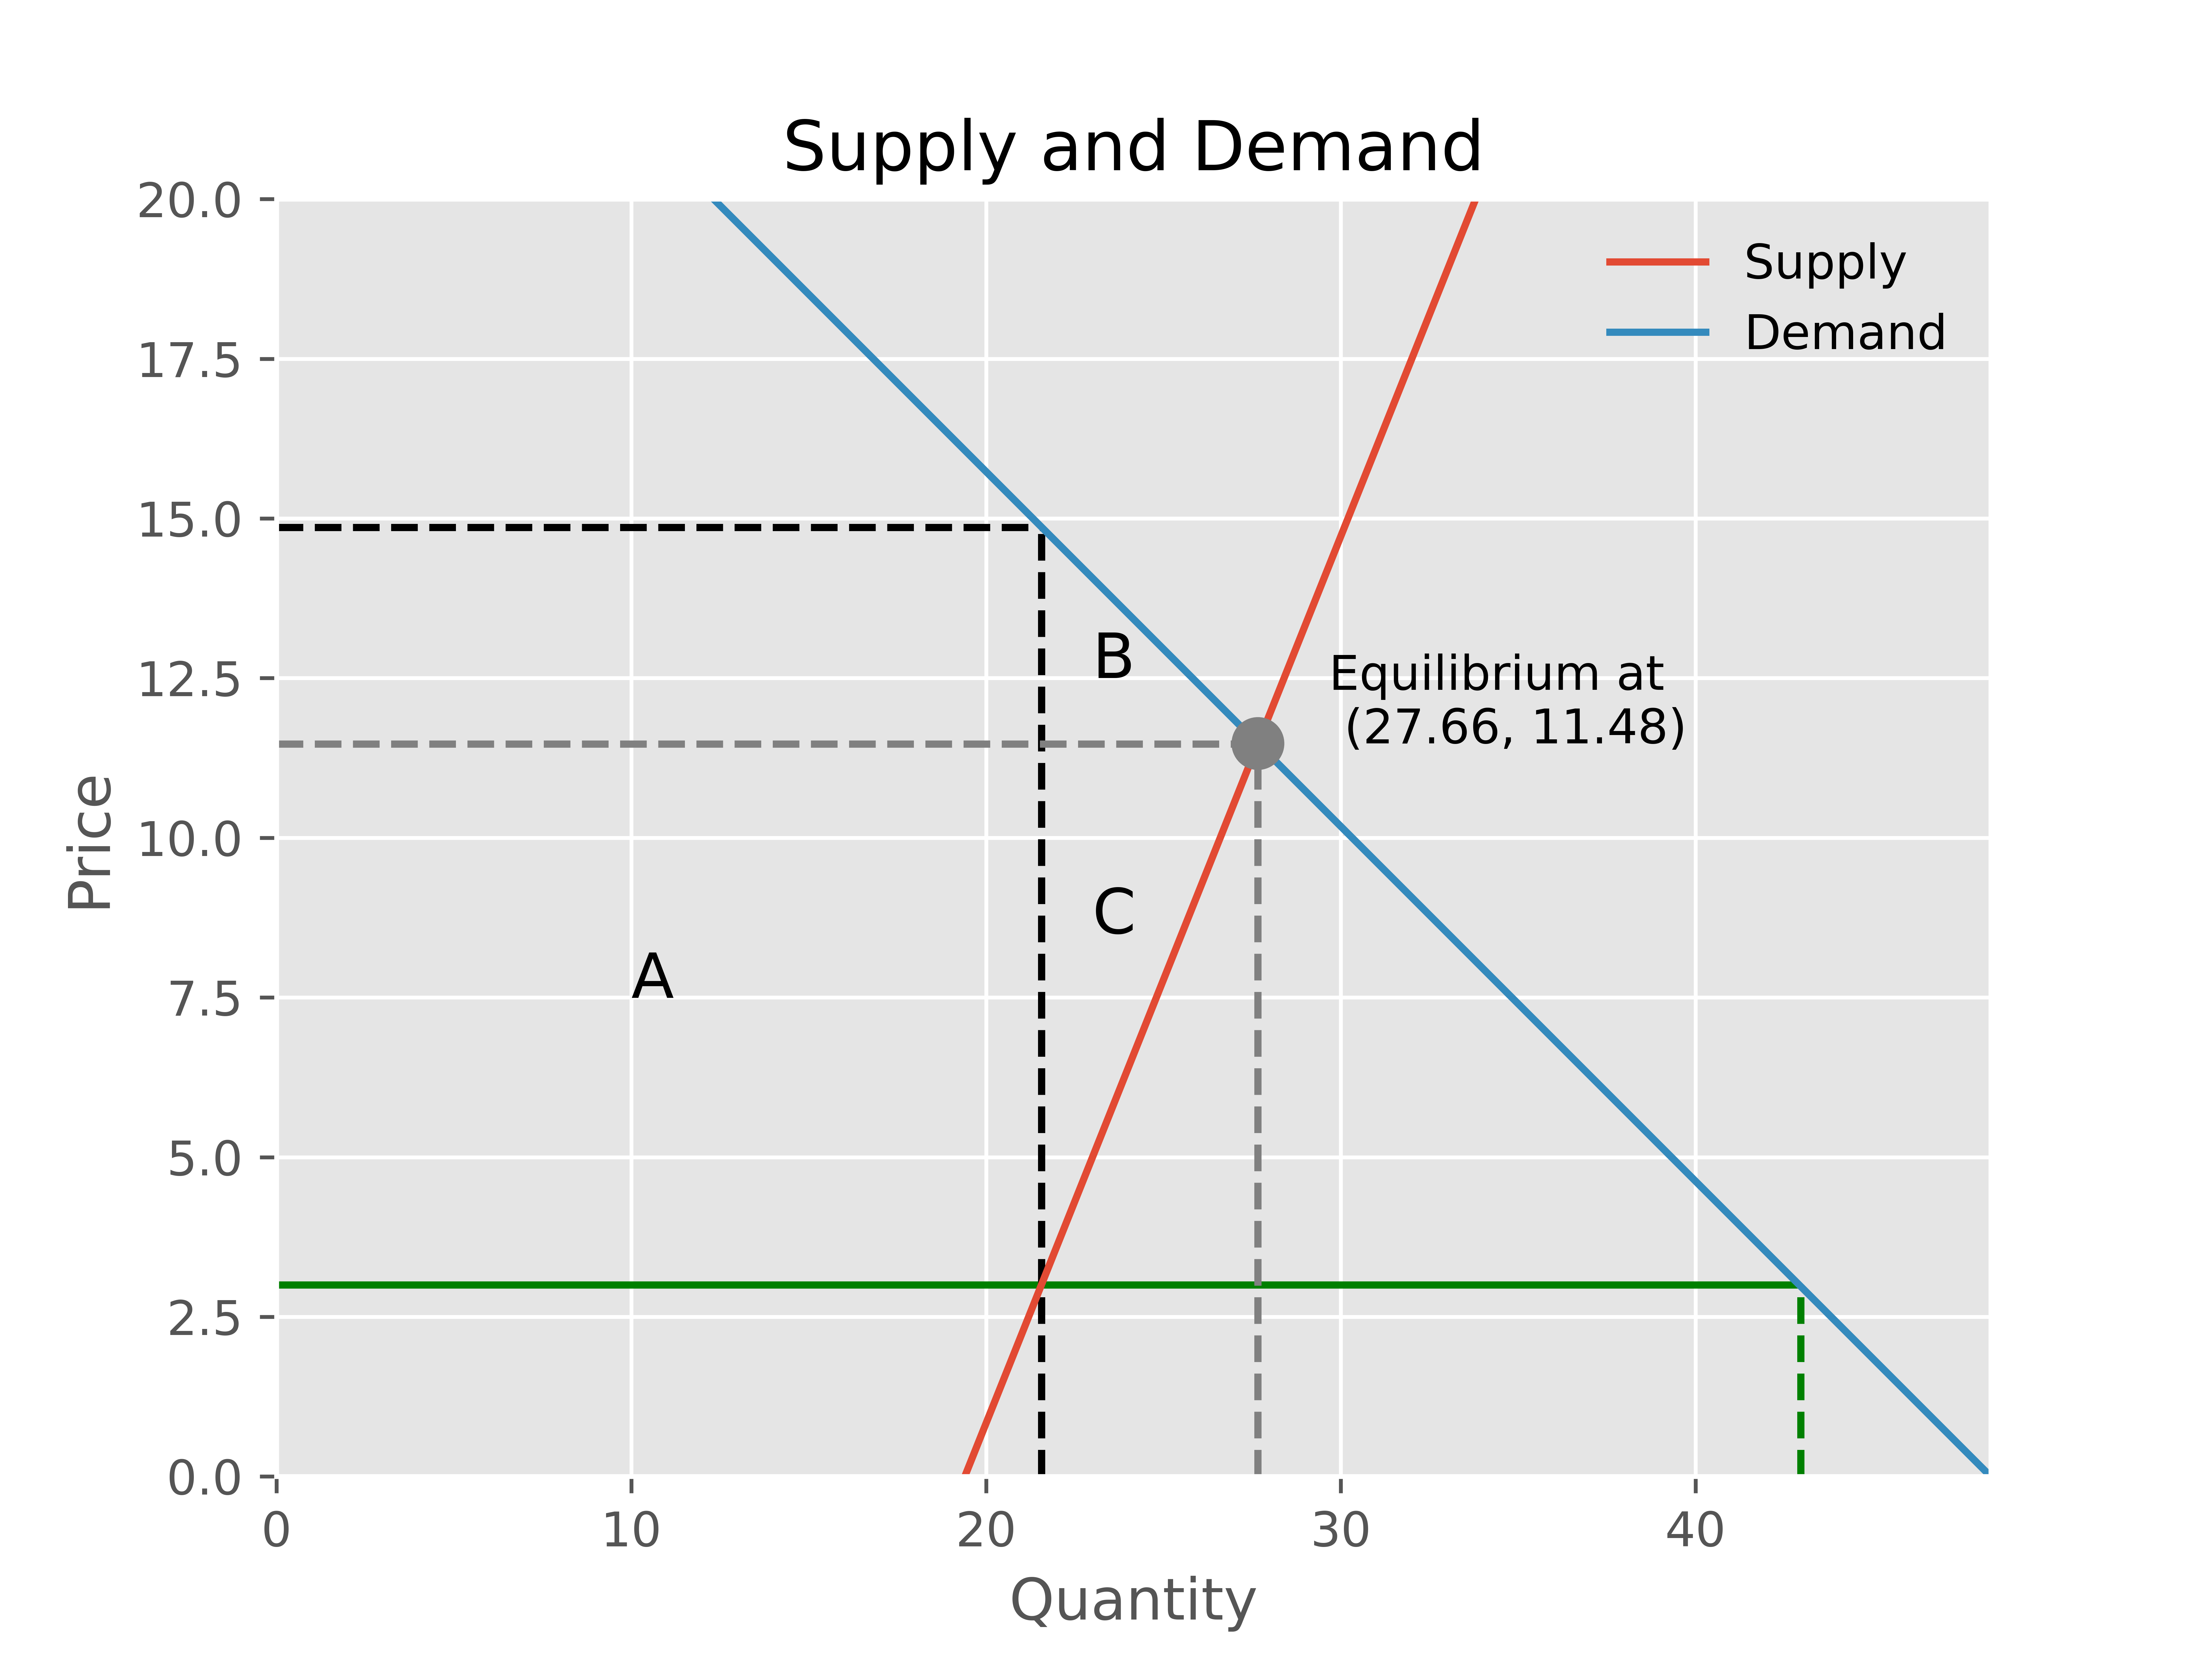
\includegraphics{curve.png}
\end{figure}

(b) Que preço de petróleo geraria um preço do gás natural de US\$ 3 no mercado livre?

\begin{gather*}
    15,90 + (0,72 \times 3) + 0,05P_P = 0,02 - (1,8 \times 3) + 0,69P_P \\
    18,06 + 0,05P_P = -5,38 + 0,69P_P \\
    \bm{P_P = 36,625}
\end{gather*}

\end{document}
